The algorithm is summarized into the following steps,
% \begin{figure}
%   \centering    
% 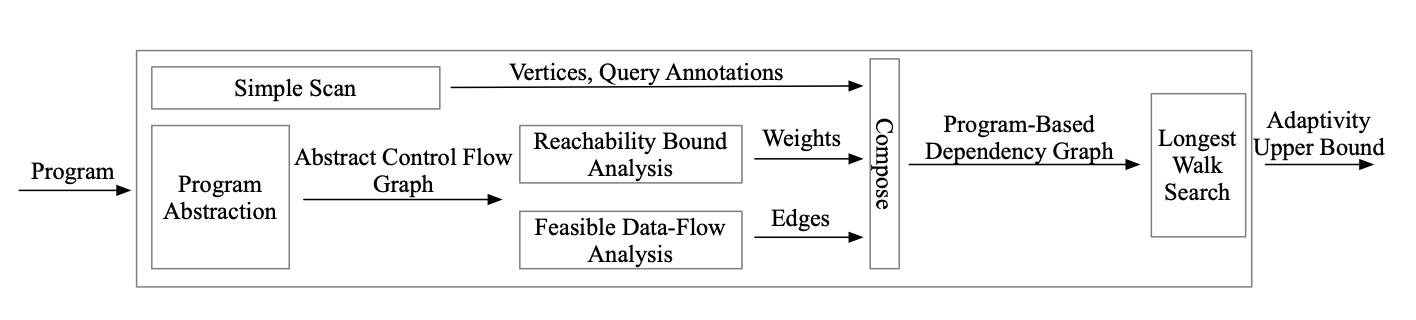
\includegraphics[width=1.0\columnwidth]{adapfun.png}
%   \vspace{-0.3cm}
%   \caption{The overview of {\THESYSTEM}}
%   \label{fig:adaptfun}
%   \vspace{-0.5cm}
% \end{figure}
%
%
\begin{enumerate}
\item  In Section~\ref{sec:abs_prog}, we first construct an abstract transition graph based on $c$, by computing an abstract transition 
for every labeled command. 
This graph is used in the following sections
for computing the path-sensitive reachability-bound of a program location.
% see Section~\ref{sec:alg_vertexgen}
\item Section~\ref{sec:refine}
refines the multiple-paths loops in the program
% this program path sensitively, 
based on the abstract transition graph.
This step transforms the multiple-paths loops into multiple loops where
the interleaving of paths is explicit.
%  which come from its abstract transition graph.
\item Section~\ref{sec:lbcompute} computes the local bound 
\footnote{\textbf{ranking function} is the named used in \cite{SinnZV14}
and \textbf{local bound} is the name used in \cite{ZulegerGSV11}, \cite{sinn2017complexity}.
We refer to the two names as the same meaning in this paper.} for each edge in a program's abstract transition graph,
and estimates the upper bounds on each local bound's maximum value and every edge's execution times path-insensitively.
% path-insensitive reachability upper bound for every while loop command in $c$.
\item Section~\ref{sec:outinalg} computes
the upper bound for the execution times of each path in a refined program locally, named \textbf{Outside-In} bound.
% path-sensitive local bounds.
\item Section~\ref{sec:inoutalg}
% performs the \textbf{Inside-Out} algorithm and 
computes the upper bound on the execution times for
every distinct path in a refined program globally, named \textbf{Inside-Out} bound.
% abstract transition graph.
\item Section~\ref{sec:psrbcompute} computes the path-sensitive reachability-bound for every program point
%  in this program 
based on the above results.
%  by
%  ?summarizing 
% the path-sensitive reachabilitybound of each edge on the abstract transition graph.
% \item The Section~\ref{sec:reachabilitybound_algorithm} computes program's reachability bound in two steps as follows.
\end{enumerate}

\subsection{Abstract Transition Graph}
\label{sec:abs_prog}
% \textbf{Step 1: Program Abstract Execution Control Flow Graph}

An \emph{Abstract Transition Graph}, $\absG(c)$ for a program $c$ is composed of
a vertex set $\absV(c)$ and an edge set $\absE(c)$, $\absG(c) \triangleq (\absV(c), \absE(c))$.
\\
Every 
vertex $l \in \absV(c)$ is a program point $l$ corresponding to the command with label $l$ in $c$, which is unique.
% We also call the unique label as program point.
% corresponds to a program point $l$, which is a unique
% label of a command in this program.
% $\absV(c)$ is the set of $c$'s all program points,
\\
Each edge $(l \xrightarrow{dc} l') \in \absE(c)$ is an abstract transition
between two program points $l, l'$. 
There is an edge from $l$ to $l'$ if and only if
the command with label $l'$ can execute right after the execution of the command with label $l$.
% if and only if there is a control flow between two program points.
Each edge is annotated by a constraint $dc \in \dcdom^{\top}$, which is generated from the command with label $l$.
This constraint describes the abstract execution of the command with $l$. 
The edge set is constructed in three steps summarized as follows (with detail in Appendix).
\begin{enumerate}
    \item Computing \textbf{constrains} over the expression for every program's labeled command,
  which is used as the annotation of an edge.
  Its domain $\dcdom^{\top}$ is composed of the \emph{Difference Constraints} $DC(\mathcal{VAR}  \cup \constdom)$,
  the \emph{Boolean Expressions} $\booldom$ and $\top$.
%
\begin{itemize}
\item The difference constraints $DC(\mathcal{VAR}  \cup \constdom)$ is the set of all the inequality of
form $x' \leq y + v$ where $x \in \mathcal{VAR} $, 
$y \in \mathcal{VAR}$ and $v \in \constdom$.
The \emph{Symbolic Constant} set $\constdom = \mathbb{N} \cup \inpvar \cup {\infty}$
is the set of natural numbers with $\infty$ and the input variables.
% , and a symbol $Q_m$ representing the abstract value of a query request.
An inequality $x' \leq y + v$ describes that the value of $x$ in the current state is
at most the value of $y$ in the previous state plus some constant $v$.
When a difference constrain shows up as an edge annotation, $l \xrightarrow{x' \leq y + v} l'$,
% Then $x'$ 
it denotes that
the value of variable $x$
after executing the command at $l$ is at most
% and the right-hand side describes 
the value of variable $y$ plus $v$ before the execution.
For every expression in each of the label command, it is computed in three steps via program abstraction method adopted from the Section~6 in \cite{sinn2017complexity}. 
%
\item The Boolean Expressions $b$ from the set $\booldom$.
$b$ on an edge $l \xrightarrow{b} l'$ describes
that after evaluating the guard with label $l$,
$b$ holds and the command with label $l$ will execute right after.
%
\item The top constraint, $\top$ denotes true. It is preserved for $\eskip$ command.
%
\end{itemize}
    \item \textbf{Initial and final state} computation step generates two sets for each labeled command in $c$. 
  The initial state contains the
  label where this command {starts} executing, 
  and the final state is a set
  that contains the constraint of this command
  and the continuation labels after the execution of this command.
%   \\ 
 \item \textbf{abstract event} computation step generates a set of edges for the $c$, by computing the initial state and finial state interactively and recursively.
%   Each edge is a pair of initial and finial state.
\end{enumerate}

\subsection{Multiple-Path Loop Refinement}
\label{sec:refine}
Algorithm Steps:
\\
\textbf{Step1: Simple Transition Path}.
\\
% Computes the Simple Transition Paths from Constraint Program,  
% 
Simple Transition Path: $\tpath \in \paths(\absG(c))$.
\\
% For a constraint program $\absG(c)$,
A \emph{simple transition path} is a path of a constraint program, $\tpath \in \paths(\absG(c))$.
It either
\begin{itemize}
  \item contains only one loop (without any nested loop) starting from a loop header at location $l$ and go back to the same $l$;
  \item or doesn't contain a loop, starting from a loop header $l$ (or the program entrance $l_0$)
and ending with different loop header $l'$ (or the program exist $\lex$).
\end{itemize}
%
\textbf{Step2: Repeat Pattern}.
% \\
% A \emph{Repeat Pattern} ($\rprog \in \mathcal{P}({\absG(c)})$) is either a simple path or sequence of repeat patterns of this program $c$. 
% \[
%   \rpattern := \tpath ~|~ \rprepeat(\rpattern) ~|~ \rpattern; \rpattern
% \]
% Every $\rprog'$ with the annotation $\rprepeat$, (for example, $\rpattern = \rprepeat(\rpattern')$)
% can consecutively execute at least twice.
% Every two sub-repeat patterns following each other in a $\rprog$ can execute in sequence, for example in $\rpattern = \rpattern_1; \rpattern_2$,
% $\rpattern_2$ can execute after $\rpattern_1$.
% Every sub-repeat patterns in the sequence are distinct.
%  \\
% Through Path-Sensitive Refinement / Contextualization algorithm in \cite{GulwaniJK09, ZulegerGSV11},
% this step computes the repeat patterns over all \emph{simple transition path}s.
% \\
% \begin{defn}[Repeat Pattern of A Program]
%   \label{def:repeat-pattern}
%   Given a constraint program $\absG(c)$,
%   $\rpattern(c)$ is a \emph{Repeat Pattern} of $\absG(c)$ if and only if, it is a simple path or
%   a sequence of \emph{repeat pattern}
%   has the following syntax
%   \[
%     \rpattern := \tpath ~|~ \rprepeat(\rpattern) ~|~ \rpattern; \rpattern
%   \] 
%   and satisfying,
%   \begin{itemize}
%   \item every sub-repeat pattern $\rpattern' \in \rpattern(c)$ with the annotation $\rpattern$
%   can consecutively execute twice
%   %  when executing this program $c$ 
%   w.r.t. some initial trace,
%   \item every sub-repeat patter in a sequence is distinct, i.e., $\rpattern(c) = \rpattern_1; \cdots; \rpattern_n$ and 
%   % $\rpattern_i, \rpattern_j \in \rpattern_1; \cdots; \rpattern_n$, 
%   $\rpattern_i \neq \rpattern_j$ for every $i, j = 1, \cdots, n$,
%   \item and every two continuous sub-repeat patters in a sequence can execute after each other w.r.t some initial trace,
%   i.e., $\rpattern(c) = \rpattern_1; \cdots; \rpattern_n$ and for every $i = 1, \cdots, n$,
%   $\rpattern_i$ can execute after $\rpattern_{i - 1}$ under some initial trace.
%   \end{itemize}
% \end{defn}
%
\textbf{Step3: Refined Program}.
% \\
\begin{defn}[Refined Program of A Program]
  Given a constraint program $\absG(c)$,
  its \emph{Refined Program} is either a repeat pattern, or a set of refined program, or sequence of refined program has
  the following syntax,
  \[
    \rprog :=  \rprepeat ~|~ \rpchoose\left\{\rprog\right\} ~|~ \rprog; \rprog.
  \]
  It satisfies that for every sub refined program $\rprog' \in \rprog$
  % $\rprog = \rprog_1, \cdots; \rprog_n$ and
  % $\rprog_i = \{\rpattern_{0}; \cdots; \rpattern_{i_n}\}$, $n, i_n \in \mathbb{N}$ and
  \begin{itemize}
  \item if
   $\rprog' = \rpchoose\left\{\rprog_1, \cdots, \rprog_m \right\}$,
   then all the $\rprog_1, \cdots, \rprog_m$ have the same starting and ending label,
  \item if $\rprog' = \rprog_1; \rprog_2$, then
  % and for every $\rpattern_1 \in \rprog_i$ and $\rpattern_2 \in \rprog_{i + 1}$,
  $\rprog_1$'s ending label is the same label as $\rprog_2$'s starting label.
  \end{itemize}
\end{defn}
%
%  annotation for two branches of $\eif$.
% them into
%  of this loop header
%s
\textbf{Theorem Guarantee.}
Soundness of the refinement.
\subsection{Local Bound Computation}
\label{sec:lbcompute}
Steps:
\\
\textbf{Step1: Variable Constraint Collection:}
Identify the abstract events where each variable is increased, decreased and reset:
\\
$\inc: \mathcal{VAR} \to \mathcal{P}(\absE(c)) $
the set of the abstract events where the variable increase.
\\
$\inc(x) = \{(e, c) | e = (l, x' \leq x + c, l') \land e \in \absE(c)\}$
\\
$\reset: \mathcal{VAR} \to \mathcal{P}(\absE(c)) $
The set of the abstract events where the variable is reset.
\\
$\dec: \mathcal{VAR} \to \mathcal{P}(\absE(c)) $
The set of abstract events where the variable decrease.
\\
\textbf{{Step2: Assign Ranks / Local Bound to Edges}}
$\locbound: \absE(c) \to \mathcal{VAR} \cup \constdom$.
 \\
\textbf{Step3: Ranks / Local Bounds Estimation}
Estimating the bounds on the (ranks'/ local bounds') maximum value.
% , the 
\\ 
$ \varinvar: \mathcal{VAR} \cup \constdom \to \mathcal{A}_{\lin}$
% \\
% $\absclr: \absE(c) \to \mathcal{A}_{\lin}$
\\
$Incr(x) \triangleq \sum\limits_{(e, c) \in \inc(x)}\{\absclr(\absevent) \times v\}$
\\
Then estimate the bounds on the iteration times
% of the ranks / local bounds 
for each edge in a path-insensitive fashion.
% \\
% computing the loop bound in a path-insensitive way as the base step.
% \\ 
% $ \varinvar: \mathcal{VAR} \cup \constdom \to \mathcal{A}_{\lin}$
\\
$\absclr: \absevent \to \mathcal{A}_{\lin}$
\\
\textbf{Theorem Guarantee.}
Soundness of the Path-Insensitive Local Bound / Rank Estimation.
%  Require Variable Bound Computation.
\subsection{Outside-In Algorithm}
\label{sec:outinalg}
For the refined program $\rprog \in \mathcal{RP}$, the \textbf{Outside-In Algorithm} ($\outinB: \rprog \to \mathcal{A}_{in}$)
computes the \emph{OutIn} bound on the iteration numbers of every repeat pattern in this program.
\\
It is called \emph{OutIn} bound because for a repeat pattern $\rpattern$ nested
in another repeat pattern $\rpattern' = \rprepeat(\rpattern)$,
this value only bounds the iteration number of $\rpattern$ inside $\rpattern'$ by assuming $\rpattern'$ executes once.

\highlight{\textbf{Notations / Operators:}}
\\
The \emph{State}: 
$\absstate \in \mathcal{P}(\dcdom^{\top})$ : conjunctions of the edge annotations.
%  constraints.
\\
For a refined program ($\rprog$), there are the 
\\
\emph{Initial State} ($\rfinit(\rprog)$), 
\emph{Final State} ($\rffinal(\rprog)$), and \emph{Next State} ($\rfnext(\rprog)$)  $\in \absstate$.
% The \emph{Initial State}: $\rfinit : \rprog \to \absstate $.
\\
The \emph{Variable Grade Decedent}: $\varGD : \rprog \to \mathcal{A}_{in}$, is the set of the variables' variation in one iteration;
% The \emph{Initial State}: $\rfinit : \rprog \to \absstate $.

\highlight{\textbf{Omitted Computations:}}
\\
Computing the $\outinB$ bound for a refined program $\rprog$. 
\\
$\outinB(\rpchoose\{\rprog_i\}) =  \max\{\outinB(\rprog_i)\}$
\\
$\outinB(\rprepeat\{\rprog\}) =  \frac{\rfinit(\rprog) - \rffinal(\rprog)}{\varGD(\rprog)}$
\\
$\outinB(\rpseq(\rprog_1, \rprog_2)) =  \outinB(\rprog_1)+ \outinB( \rprog_2)$
\\
$\outinB(\tpath) =  1$.
\\
The computations of the operations: $\rfinit(\rprog)$,
$\rffinal(\rprog)$ $\rfnext(\tpath)$ and $\varGD : \rprog \to \mathcal{A}_{in}$ is in Appendix.
Equivalent result can be computed for $\outinB(\rprepeat\{\rprog\})$ by alternative computation method from paper \cite{GulwaniJK09} while in-efficiently.
\subsection{Inside-Out Algorithm}
\label{sec:inoutalg}
For the refined program $\rprog \in \mathcal{RP}$, the \textbf{Inside-Out Algorithm}
computes the reachability-bound on the execution numbers for every simple transition path $\tpath$ in this program $\rprog$,
through the following steps.
%
\begin{enumerate}
  \item \emph{Repeat Chain Bound:} $\rpchB(l, \tpath, \rprog) \in \mathcal{A}_{in}$.
  \\
  For every transition path $\tpath$ in a refined program $\rprog$,
  its \emph{Repeat Chain Bound} is the
  bound on its execution numbers inside its closet while loop.

  \highlight{\textbf{Omitted Computations:}}
\begin{defn}[Repeat Chain]
  \label{def:repeatchain}
For a refined program $\rprog$ and a simple transition path $\tpath$,
a \emph{Repeat Chain} $\rpch(l, \tpath, \rprog)$
is a list of repeat patterns nested in a repeat pattern with loop header annotation $l$,
%  efined program contained inside the same while loop $L$ as the $\tpath$. 
% It is computed as follows,
  % $\rpch(L_l, \tpath) \in \mathcal{P}(\rprog)$\\
\[
 \rprog_n \to \rprog_{n-1} \to \cdots \to \tpath
\]
It satisfies
 $\rprog_{i}= l : \rprepeat(\cdots, \rprog_{i - 1}, \cdots)$ and
 there isn't any nested loop header ($l'$) or $\rprepeat$ annotation between $\rprog_{i}$ and $\rprog_{i - 1}$
 for every $i = n, \cdots, 1$.
\end{defn}
%
\textbf{Repeat Chain Set}
\begin{defn}[Repeat Chain Set]
  \label{def:repeatchainset}
  For a refined program $\rprog$ and a simple transition path $\tpath$, the \emph{Repeat China Set}
  $\rpchset(l, \tpath, \rprog)$ is the set of 
  all repeat chains for $\rprog$ and $\tpath$,
  \[
    \left\{\rpch(l, \tpath, \rprog) \right\}.
 \]
\end{defn}
\textbf{Repeat Chain Bound}
\\
For every transition path $\tpath$
in its closet enclosed while loop $l$,
% $rpRB: \tpath \to \mathcal{A}_{in}$, $chsRB: (\rprog \times \tpath) \to \mathcal{A}_{in}$
% \\
% For each transition path $\tpath \in \rprog$,
% \\
% 1. First compute the path sensitive reachability choosing bound through their choose chain:
% \\
% $chsRB(\rprog_n, \tpath) = \prod\limits_{\rprog_i \in lpchain(\rprog_n, \tpath)}
% \frac{chsInit(\rprog_i, \tpath) - chsFinal(\rprog_i, \tpath)}{\varGD(\rprog_i, \tpath)}$
  \\
  $
  \begin{array}{l}
    \rpchB(l, \tpath,  \rprog) = \\
    \max \left\{ \prod\limits_{\rprog_i \in ch}  \outinB(\rprog_i) 
  ~\middle\vert~ ch \in \rpchset(l, \tpath, \rprog) \right\}
  \end{array}
  $
  \\
  \item \emph{Relative Loop Bound:} $\lpchB(l, \tpath, \rprog) \in \mathcal{A}_{\lin}$.
  \\
  For every simple transition path $\tpath$
and a loop header at location $l$ in a refined program $\rprog$,
the \emph{Relative Loop Bound} $\lpchB(l, \tpath, \rprog) \in \mathcal{A}_{\lin}$ is a symbolic expression in $\mathcal{A}_{\lin}$.
\\
This expression is a sound bound on the iteration numbers of loop $l$ relative to the simple transition path $\tpath$.
This $\tpath$'s closest enclosing loop has the loop header at $l'$ and $l'$ is nested inside the loop $l$.
\\
It estimates the iteration numbers of loop $l$ such that during these iterations, the nested loop $l'$ is executed.

%  will 
\highlight{\textbf{Omitted Computations:}}
\\
\textbf{Loop Chain}.  $\lpch(\tpath, \rprog) \in \mathcal{P}(\rprog)$.
\begin{defn}[Loop Chain]
  \label{def:loopchain}
For a refined program $\rprog$ and a simple transition path $\tpath$ in this program, the loop chain $\lpch(\tpath, \rprog)$
is
%
\[ 
\rprog_n \to \rprog_{n-1} \to \cdots \to \tpath
\]
% such that there is at least a $\rpchoose$ and isn't consecutive repeats $\rprepeat$ (i.e., at most one 
% $\rprepeat$) between any $\rprog_{i - 1}$ and $\rprog_{i}$ for $i = n, \cdots, 1$.
such that 
$\rprog_{i}= l_i : (\cdots, l_{i - 1} : \rprog_{i-1}, \cdots)$ and
 there isn't any nested loop annotation (i.e., $l'$) between $\rprog_{i}$ and $\rprog_{i - 1}$ for $i = n, \cdots, 1$.
\end{defn}
%
\highlight{
\textbf{Relative Loop Bound:}
% $\lpchB(l, \tpath, \rprog) \in \mathcal{A}_{\lin}$.
\begin{defn}[Relative Loop Bound]
  \label{def:relatedloop_bound}
For every simple transition path in a refined program $\tpath \in \rprog$
and every loop $l \in \lpch(\tpath, \rprog)$,
% where $\lpch(\tpath)  \in \rpchset(\tpath)$, 
the \emph{Relative Loop Bound} $\lpchB(l, \tpath, \rprog)$ is computed as follows,
\[
  \left\{
  \begin{array}{l}
    \rpchB(l, \tpath, \rprog)  
    \\ \qquad \rpchB(l, \tpath) \neq \bot
    \\
    \frac{\lpinit(l, \tpath) - \rffinal(\tpath)}{\lpinit(l, \tpath) - \lpnext(l, \tpath)}
     \qquad o.w.
  \end{array}
  \right\}
  \]
\end{defn}
}
The computations of the operations $\lpinit(L_i, \tpath)$ and $\lpnext(L_i, \tpath)$ are in Appendix.
%
\item The \emph{Inside-Out Bound} ($\inoutB(\tpath, \rprog) \in \mathcal{A}_{in}$).
\\
For every simple transition path $\tpath \in \rprog$,
its \emph{Inside-Out Loop Bound}
 $\inoutB(\tpath, \rprog) \in \mathcal{A}_{in}$ is 
% Compute 
the path sensitive reachability-bound on $\tpath$'s execution numbers.

\highlight{\textbf{Omitted Computations:}}
\begin{defn}[{Inside-Out Loop Bound}]
  \label{def:outin_bound}
  Given a refined program $\rprog$, for every transition path $\tpath \in \rprog$, 
  its \emph{Inside-Out Loop Bound}
  $\inoutB(\tpath, \rprog)$ is 
 % Compute 
\[
  \prod\limits_{L \in \lpch(\tpath, \rprog)} \rpchB(l, \tpath, \rprog).
% lpRB(\rprog_i, \tpath) 
% ~ \middle\vert~ l \in lp\mathcal{C}(\tpath) \right
\]
\end{defn}
% For $chain \in rpchain(\tpath)$:
% where $lpchains(\tpath)$ is set of $lpchains(\tpath)$ containing all the loop chains of $\tpath$.
\end{enumerate}
\subsection{Path Sensitive Reachability Bound Computation}
\label{sec:psrbcompute}
For every program control location $l \in \lvar(c)$, with $\rprog$ as its refined program,
%  in a program $c$,
its path-sensitive reachability-bound ($\psRB(l, \rprog)$) is a symbolic sound bound on the executing times of $l$.

\highlight{\textbf{Omitted Computations:}}
 \begin{defn}
  \label{def:label_psrb}
Given a program $c$ with its refined program $\rprog \in \mathcal{RP}$
%  with 
% \emph{Global Loop Bound} $\inoutB(\tpath)$
% computed for its every transition path $\tpath \in \rprog$  notated by $\inoutB(\tpath)$,
%  for each of its transition path $\tpath \in \rprog$ 
% with the \emph{Global Loop Bound}
% computed as above, notated by $\inoutB(\tpath)$.
the $\psRB(c, l)$ for every label $l \in \lvar(c)$ is computed as follows,
\\
\[ \psRB(c, l) = \sum\limits_{\tpath \in \rprog \land 
l \in \tpath} \inoutB(\tpath)\]
 \end{defn}
\begin{thm}[Soundness of the Path Sensitive Reachability Bound Estimation]
  \label{thm:pathsensitive_rb_soundness}
Given a program ${c}$, for every label $l$ of this program $c$ such that $(l, w) \in \exeRB(c)$, 
and any initial trace $\trace_0 \in \mathcal{T}_0(c)$ with 
% $\config{{c}, \trace_0} \to^{*} \config{\eskip, \trace_0\tracecat \vtrace} $ 
and $\config{\psRB(c, l), \trace_0} \earrow v$,
% for some generated evaluation trace $\vtrace \in \mathcal{T}$,
we have $ w(\trace_0) \leq v $.
%
\[
  \begin{array}{l}
  \forall (l, w_{t}) \in \exeRB(c),
  % (x^l, w_{p}) \in \progV, 
  \trace_0 \in \mathcal{T}_0(c), 
  v \in \mathbb{N} \st
  \\ \quad
  \config{\psRB(c, l), \trace_0} \earrow v
  \implies
  w_{t}(\trace_0) \leq v
  \end{array}
  \]
\end{thm}
%
Proof of this theorem is in Appendix.